\documentclass[hyperref=colorlinks]{beamer}
\mode<presentation>
\usetheme{iclpt}
\setbeamertemplate{navigation symbols}{}
\setbeamertemplate{headline}{
\begin{beamercolorbox}[leftskip=.2cm,rightskip=.2cm,topskip=.2cm,ht=1.1cm,dp=0.1cm,wd=\textwidth]{institute in head/foot}
  
\includegraphics[height=1cm]{icl.pdf}
  \hfill
  
\includegraphics[height=1cm]{../Pics/CMS-Color.pdf}
\end{beamercolorbox}
}
\setbeamertemplate{footline}{
\begin{beamercolorbox}[ht=.55cm,dp=0.4cm,wd=\textwidth,leftskip=.3cm]{author in head/foot}%
  \begin{minipage}[c]{5cm}%
    \usebeamerfont{author in head/foot}
    \insertshortauthor 
    \insertshorttitle
    \end{minipage}\hfill%
  \insertframenumber{} / \pageref{lastframe}
  \hfill
  \begin{minipage}{6cm}
    \hfill
  \end{minipage}
\end{beamercolorbox}%
}

\usepackage{color}
\usepackage{tabularx,colortbl}
\usepackage{graphicx}
\usepackage{pdfpages}
\usepackage{feynmp}
\usepackage{tikz}
\usetikzlibrary{calc, shapes, backgrounds,arrows,positioning}
\DeclareGraphicsRule{*}{mps}{*}{}

\title{\vspace{-0.2cm} VBF Higgs to Invisible}
\subtitle{HIG-14-038, AN-14-243\vspace{-0.7cm}}
\author[]{}%\underline{P. Dunne}} % A.M. Magnan and A. Nikitenko Joao Pela with \\ R. Aggleton, J. Brooke: Bristol \\ C.Asawangtrakuldee, Q.Li: Peking \\ P. Srimanobhas: Chulalongkorn \\ S. Kumar, K. Mazumdar: Mumbai}
\titlegraphic{
  \vspace{-0.7cm}
  %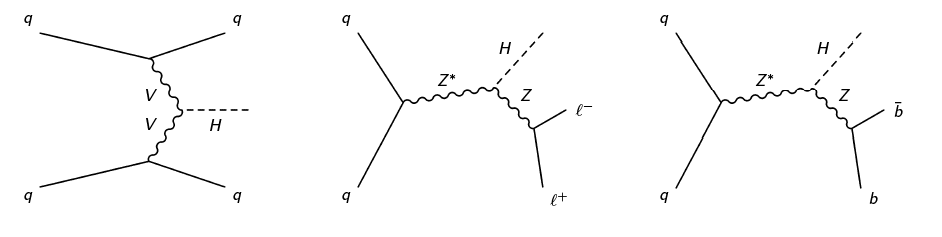
\includegraphics[width=\textwidth]{TalkPics/invcomb021213/feyndiags}
  %% \begin{fmfgraph*}(100,70)
  %%         \fmfleft{i1,i2}
  %%         \fmfright{o1,o2,o3}
  %%         \fmf{fermion}{i1,v1,o1}
  %%         \fmf{fermion}{i2,v2,o3}
  %%         \fmf{phantom,tension=4/5}{v1,v2}
  %%         \fmffreeze
  %%         \fmf{photon,label=$W,,Z$}{v1,v3}
  %%         \fmf{photon,label=$W,,Z$}{v2,v3}
  %%         \fmf{dashes}{v3,o2}
  %%         \fmflabel{$q$}{i1}
  %%         \fmflabel{$q$}{i2}
  %%         \fmflabel{$q$}{o1}
  %%         \fmflabel{$q$}{o3}
  %%         \fmflabel{$H$}{o2}
  %%       \end{fmfgraph*}
}
\date{}
\begin{document}
\begin{fmffile}{higgsexoupdatefeyndiags}
\tikzstyle{every picture}+=[remember picture]

%TITLE PAGE
\section{Title}
\begin{frame}
  \titlepage
  
\end{frame}

\begin{frame}
  \frametitle{Overview}
  \begin{block}{Reminder}
    \begin{itemize}
    \item 
    \end{itemize}
  \end{block}
  \begin{block}{New Today}
    \begin{itemize}
    \item 
    \end{itemize}
    \end{block}
\end{frame}

\begin{frame}
  \frametitle{Higgs Portal DM interpretation - recap}
  \begin{block}{}
    \begin{itemize}
    \item For prompt paper made a DM limit using EFT described \href{http://www.sciencedirect.com/science/article/pii/S0370269312001037}{here}
    \end{itemize}
  \end{block}
  \centering
  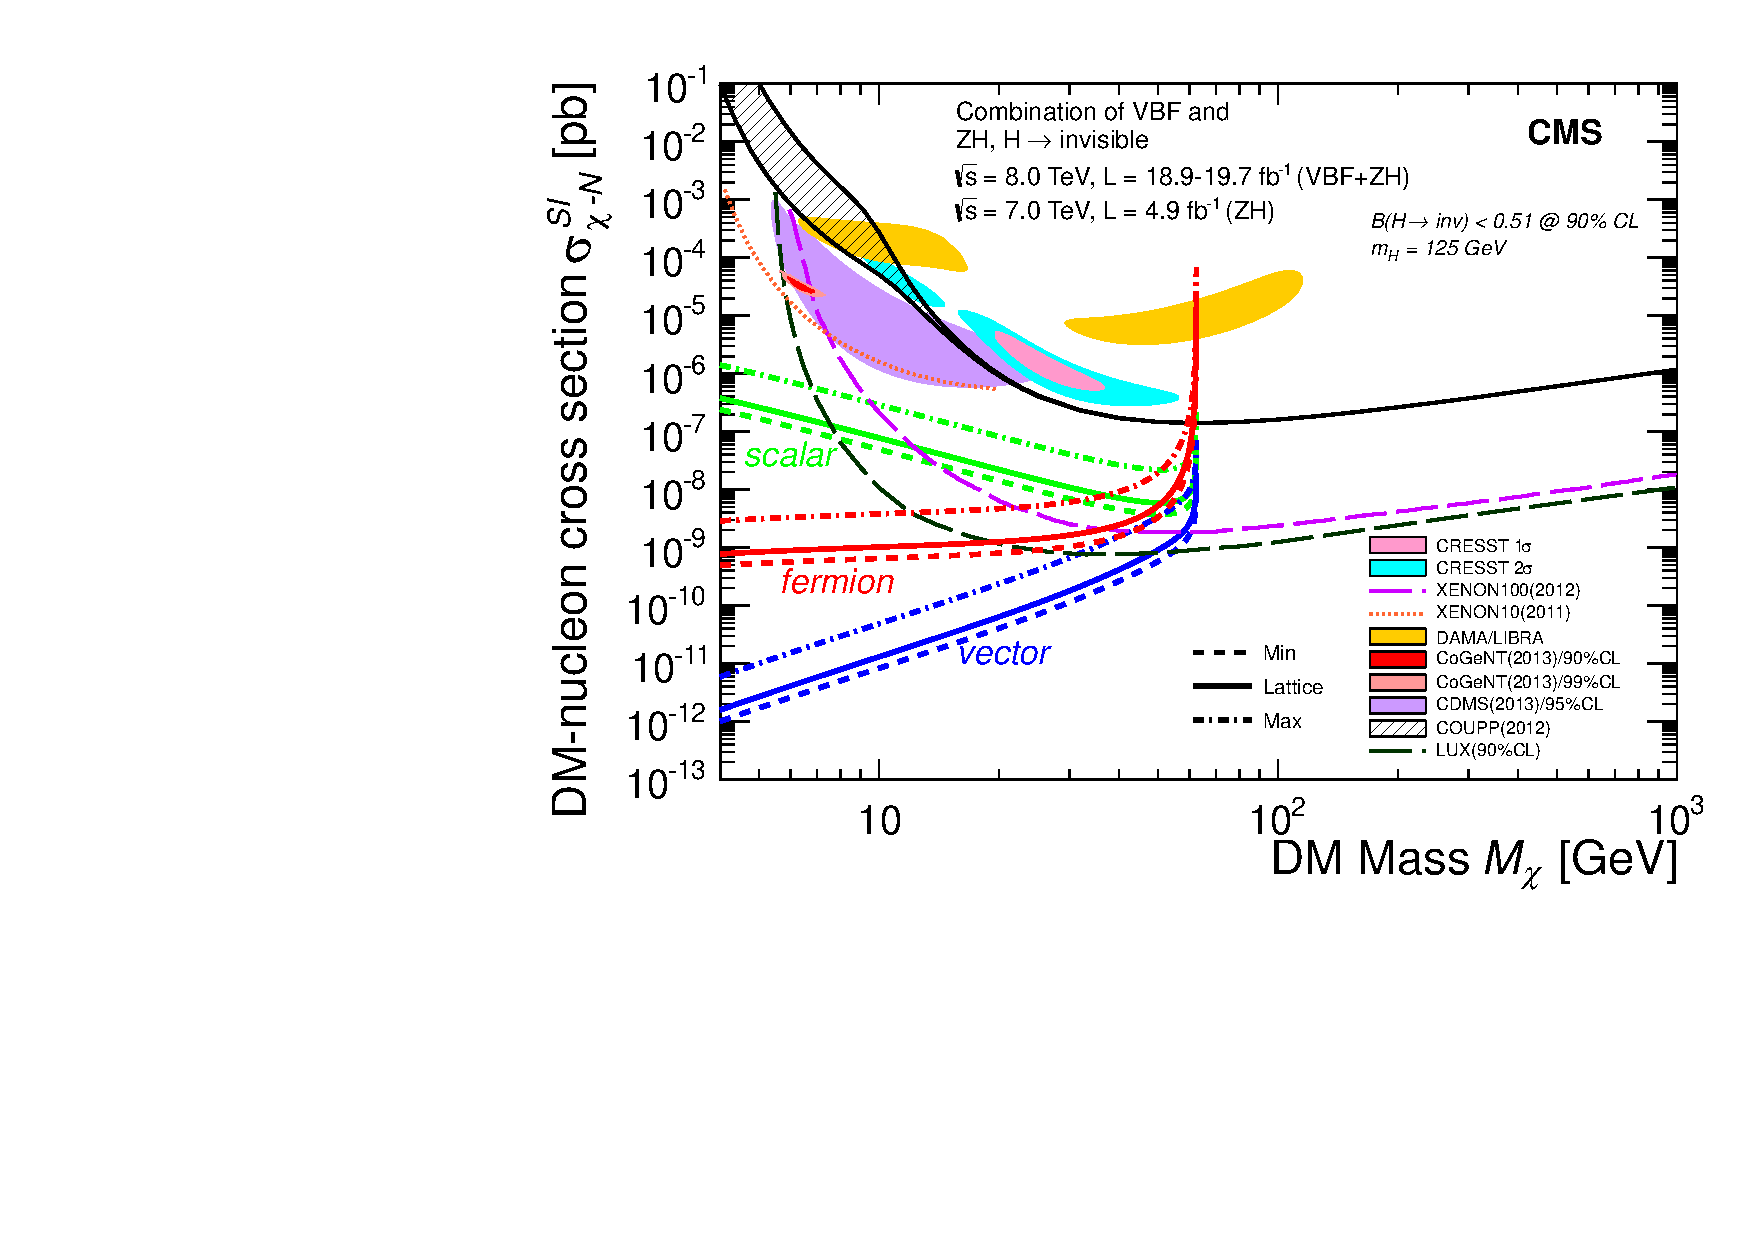
\includegraphics[width=.5\textwidth]{TalkPics/dmandqcd010615/promptdmnucleonlimit.pdf}
\end{frame}

\begin{frame}
  \frametitle{Scalar}
  \begin{block}{}
    \begin{itemize}
    \item %!!ALL FINE QUOTE OXFORD PROCEEDINGS AGREEMENT WITH DJOUADI
    \end{itemize}
  \end{block}
\end{frame}

\begin{frame}
  \frametitle{Fermion}
  \begin{block}{}
    \begin{itemize}
    \item %!!PROBLEM IN INTERPRETATION OF EFT AND RENORMALISABILITY
    \item %!!QUOTE OXFORD PROCEEDINGS MIXING MODEL AND DIFFERENT MODEL IN DM FORUM WRITEUP
    \item %!!ALSO ARXIV 1212.2131
    \end{itemize}
  \end{block}
\end{frame}

\begin{frame}
  \frametitle{Vector}
  \begin{block}{}
    \begin{itemize}
    \item %!!NOT MENTIONED IN OXFORD OR DM FORUM PROCEEDINGSFIND MORE DETAILS
    \item %!!STATED NOT GAUGE INVARIANT IN ARXIV 1412.0258
    \item %!!ALSO ARXIV 1212.2131
    \end{itemize}
  \end{block}
\end{frame}

\begin{frame}
  \frametitle{Higgs Portal DM interpretation - update}
  \begin{block}{}
    \begin{itemize}
    \item Used direct detection data from \href{dmtools.brown.edu:8080}{Brown DM tools}
    \item Use 90\% CL observed limit from HIG14038 result: 0.4048
    \item Left plot has three values of fN as in paper
    \item Right plot is prompt (dashed) vs parked plus EXO (solid)
    \end{itemize}
  \end{block}
  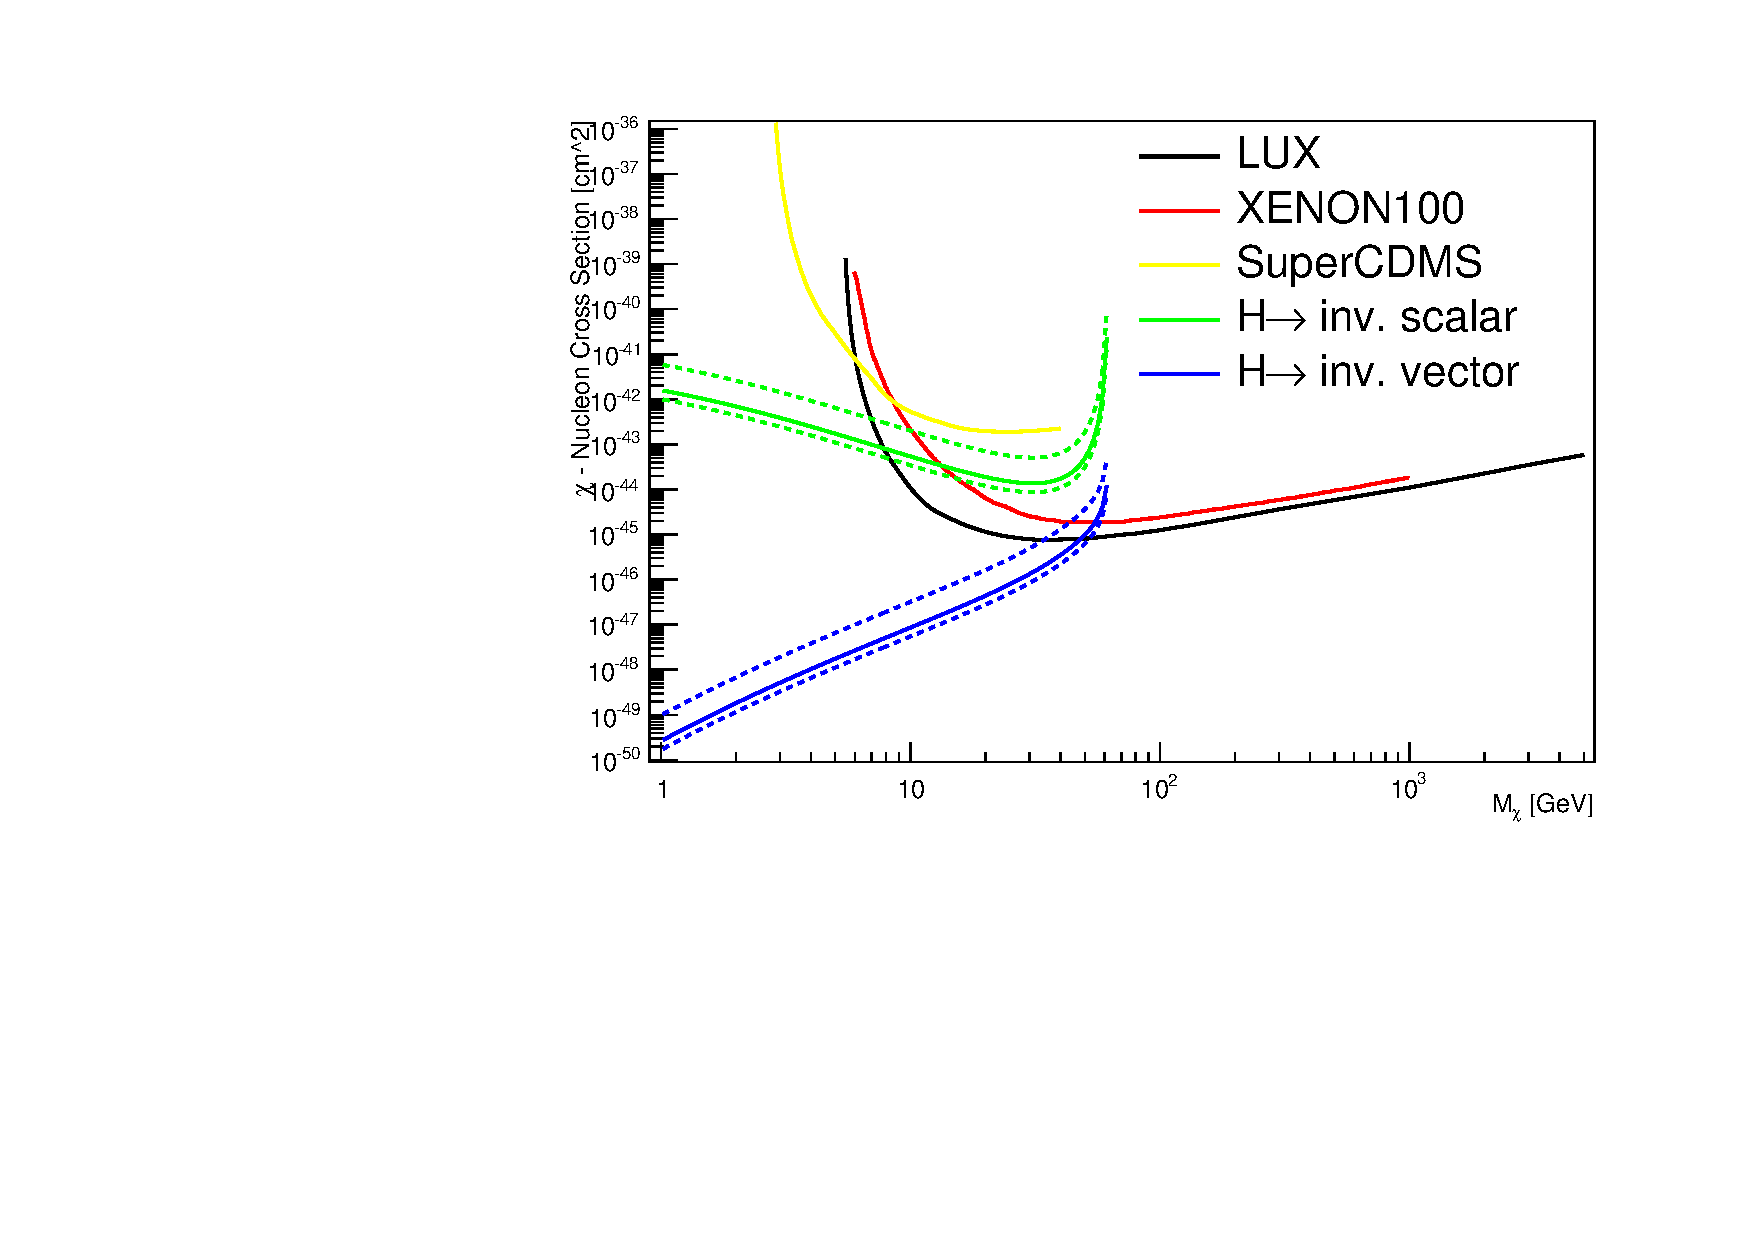
\includegraphics[width=.5\textwidth]{TalkPics/dmandqcd010615/DMplot.pdf}
  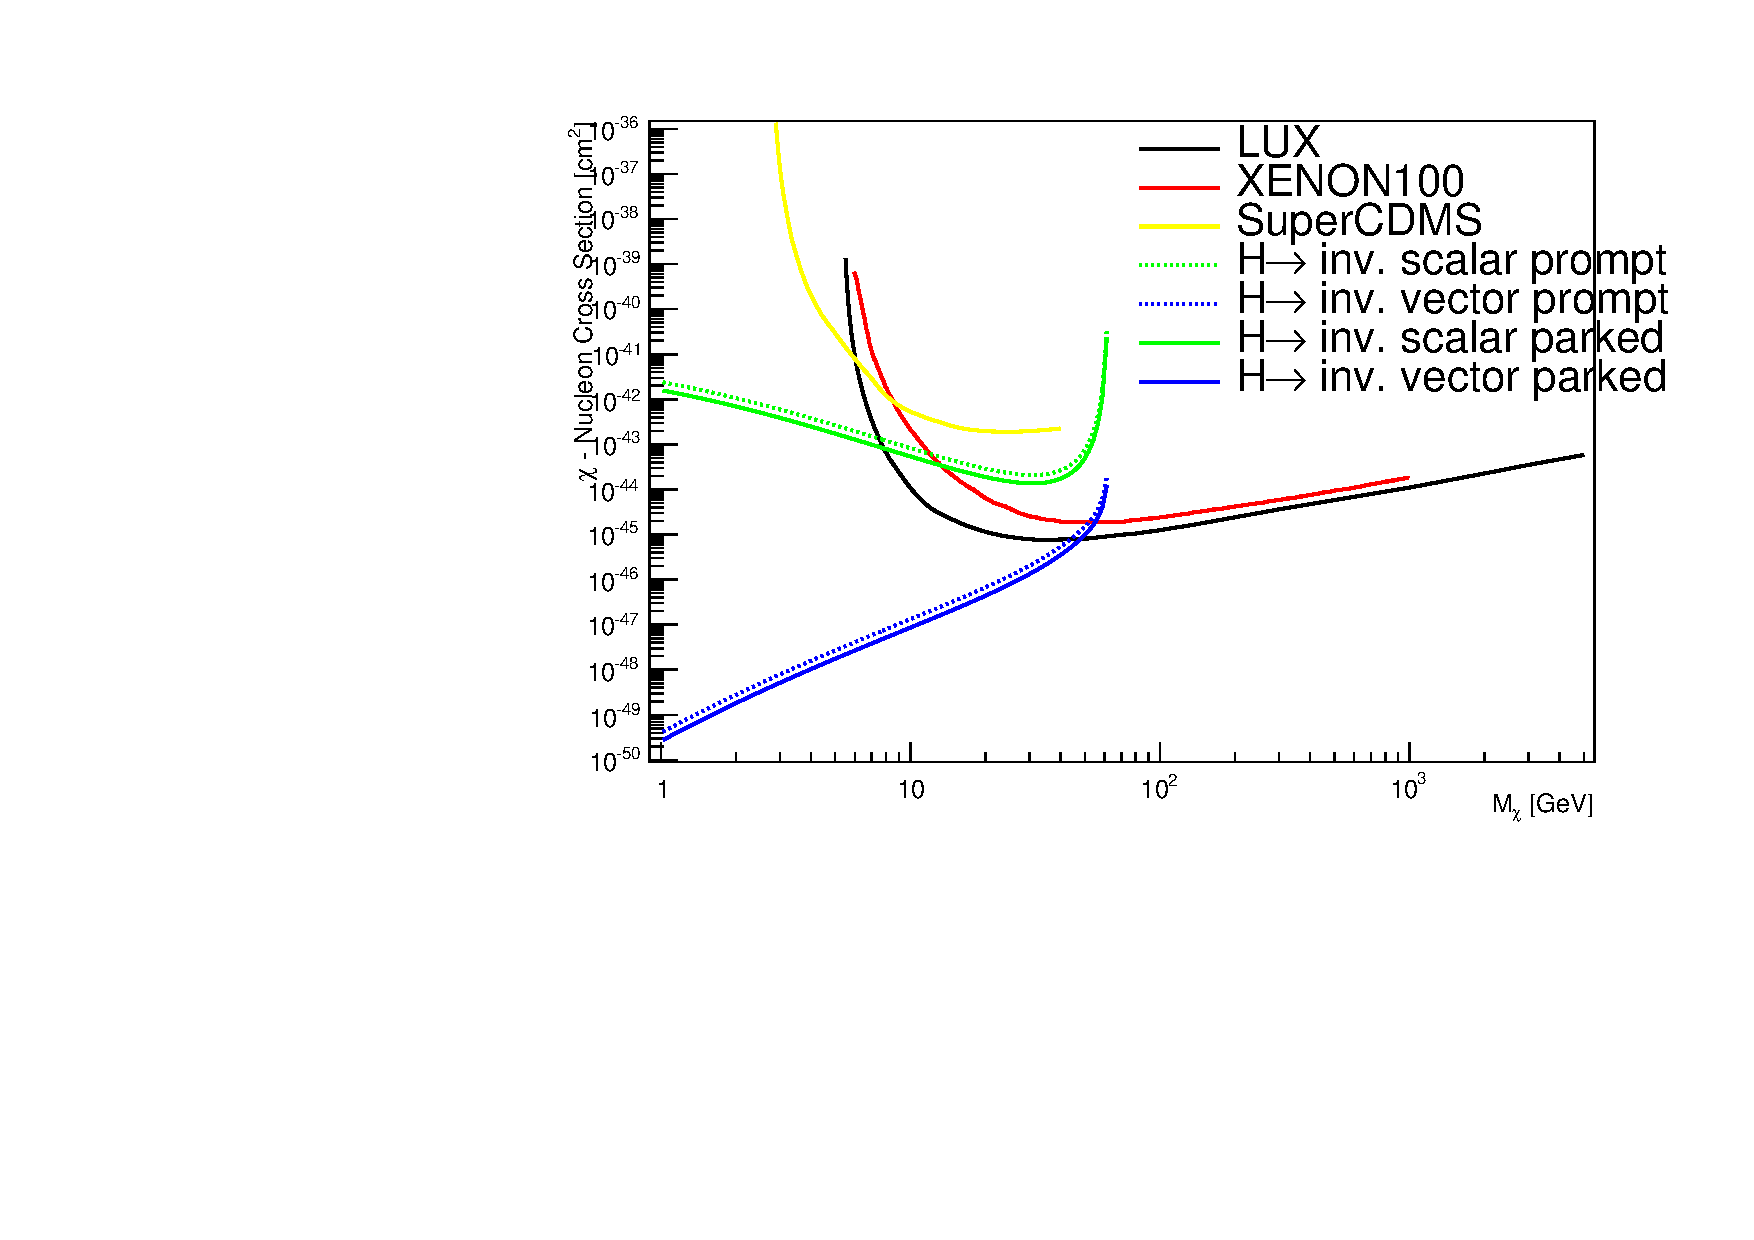
\includegraphics[width=.5\textwidth]{TalkPics/dmandqcd010615/DMplotpromptvsparked.pdf}
\end{frame}

\begin{frame}
  \label{lastframe}
  \begin{block}{Summary}
    \begin{itemize}
    \item First look at QCD samples:
    \item[-] Limited stats especially in run 1 so hard to draw conclusions
    \item[-] Also neither set models fake met so we will still need Joao's samples
    \item DM plot remade:
    \item[-] Double checking validity of scalar and vector lines
    \item[-] Can add other experiments if desired
    \item Combination with EXO:
    \item[-] Synchronising with Nick
    \item[-] PAS waiting on approval of EXO result
    \end{itemize}
  \end{block}
\end{frame}

\begin{frame}
  \frametitle{Backup}
\end{frame}

\end{fmffile}
\end{document}
